\documentclass[11pt,a4paper]{article}
\usepackage[hyperref]{emnlp2018}
\usepackage{times}
\usepackage{latexsym}
\usepackage{url}

\usepackage{amsmath}
\usepackage{amssymb}
\usepackage{bm}
\usepackage{booktabs}
\usepackage{caption}
\usepackage{CJKutf8}
\usepackage[inline,shortlabels]{enumitem}
\usepackage[T1]{fontenc}
\usepackage{footnote}
\usepackage{graphicx}
\usepackage[utf8]{inputenc}
\usepackage{multirow}
\usepackage{pifont}
\usepackage{subcaption}
\usepackage{tikz}
\usepackage{verbatim}
\usepackage{wrapfig}
\usetikzlibrary{fit,positioning}
\makesavenoteenv{table}
\makesavenoteenv{tabular}

\aclfinalcopy % Uncomment this line for the final submission
%\def\aclpaperid{***} % Enter the acl Paper ID here

%\setlength\titlebox{5cm}

%\renewcommand{\baselinestretch}{1.04}

\newcommand{\ensuretext}[1]{#1}
\newcommand{\mycomment}[3]{\ensuretext{\textcolor{#3}{[#1 #2]}}}
\newcommand{\ammarker}{\ensuretext{\textcolor{blue}{\ensuremath{^{\textsc{A}}_{\textsc{M}}}}}}
\newcommand{\am}[1]{\mycomment{\ammarker}{#1}{blue}}
\newcommand{\cjdmarker}{\ensuretext{\textcolor{red}{\ensuremath{^{\textsc{C}}_{\textsc{D}}}}}}
\newcommand{\cjd}[1]{\mycomment{\cjdmarker}{#1}{red}}
\newcommand{\gnmarker}{\ensuretext{\textcolor{green}{\ensuremath{^{\textsc{G}}_{\textsc{N}}}}}}
\newcommand{\gn}[1]{\mycomment{\gnmarker}{#1}{green}}
\newcommand{\ignore}[1]{}
\newcommand{\cmark}{\ding{51}}%
\newcommand{\xmark}{\ding{55}}%
\newcommand{\pluseq}{\mathrel{+}=}

\title{Monte-Carlo Tree Search for Inference in NLP}

\author{Austin Matthews \and Graham Neubig \\
  Language Technologies Institute \\
  Carnegie Mellon University \\
  {\tt \{austinma,gneubig\}@cs.cmu.edu} \\\And
  Chris Dyer \\
  DeepMind \\
  {\tt cdyer@google.com} \\}
\date{}

\hypersetup{draft}
\begin{document}
\maketitle

\begin{abstract}
Many NLP algorithms rely on beam search to attempt to find a globally optimal
hypothesis in the forest of possibilities produced by a locally normalized
sequential model. In this work we show that Monte-Carlo Tree Search (MCTS) can
be used as a drop-in replacement for Beam Search to provide both direct
accuracy gains and additional flexibility. Said flexibility may admit
previously untractable problem-specific approaches that yield further
improvements.

While most of the techniques discussed are abstract and applicable to many NLP
tasks, we demonstrate improvements on a machine translation task, resulting in
gains of up to 3.81 BLEU points over a beam search baseline.
\end{abstract}

\section{Introduction}
\label{sec:intro}
Many tasks in natural language processing, such as parsing, language modelling,
speech recognition, and machine translation, lend themselves to sequential
algorithms. Such algorithms typically begin in some initial \emph{state} (e.g.
an empty string, or a bare \textsc{root} node) and use an locally normalized
model to choose its next \emph{action} (e.g. emit word $w$, or take parsing
transition $t$). To get a full transcript, parse tree, or translation then
requires a non-trivial search to find a single hypothesis that globally
maximizes a scoring function. In the NLP world to date the most popular search
algorithm has been \emph{beam search}
\cite{koehn2004pharaoh,bahdanau2014neural,vinyals2015grammar,
vaswani2017attention}.

Monte-Carlo Tree Search (MCTS), on the other hand, is a search algorithm most
commonly used by game-playing programs. In particularly excels for games where
\begin{enumerate*}[(a)]
\item evaluating who has the advantage in a partially played-out position is
difficult,
\item the branching factor is large, and 
\item actions taken now show complex interactions with later actions.
\end{enumerate*}
MCTS has enjoyed particularly large
success in the Go AI community \cite{abramson1987model, brugmann1993monte,
silver2017mastering}.

Many NLP tasks, such as machine translation, can be seen as single player games in which
the single player attempts to search for a series of actions that maximizes a final score.
Furthermore, such tasks exhibit all three of the above properties, and thus lend themselves
nicely to MCTS-based solutions.

\section{Beam Search}
\label{sec:beam_search}
In beam search (with beam width $k$), the algorithm begins in its initial state
$s_0$ and queries its model for the $k$ actions that seem the most promising
locally. It then creates new nodes in its search tree for each of these $k$
children and again queries its model for the $k$ most promising actions from
each child state. Of the $k^2$ leaf nodes now in the search tree, the top $k$
are kept and all others are discarded and searched no further. The algorithm
continues this process recursively; at each step it has (up to) $k$ states to
expand, gets the locally best $k$ actions for each, and then keeps the top $k$
of the resulting $k^2$ candidate nodes.

While beam search is a strong baseline, and is the most common decoding
algorithm used for generation tasks (e.g. MT, action-based parsing, language
modelling), it is not without drawbacks.

First, beam search constrains each node in its search graph to have the same
fan out. The algorithm searchs $k$ child nodes no matter what, including from
nodes where the neural network is very confident in what the next word will be
(i.e. where the distribution over potential next actions has very low entropy).
Conversely, it can \emph{only} search $k$ child nodes, even if the entropy over
children is very high.

Second, it relies on a local scoring function, where the underlying model takes
a node and predicts, given only its previously-generated context, the next word
in the output sequence. This means that beam search can never leverage
information about what occurs later in the sentence, or about the global
quality of its output. In the context of neural machine translation, this leads
to the output of beam search being very fluent, but often unfaithful to the
source sentence. Furthermore, output tends to be shorter than desired, leading
to depressed BLEU scores \cite{koehn2017six}.

\section{Monte-Carlo Tree Search}
\label{sec:mcts}
Monte-Carlo Tree Search also begins from an initial state $s_0$ and searches
for the most promising hypothesis from the huge search tree. In theory MCTS
does not even need a local model to choose its next action, though in practice
using one is highly advised. Such a model is used as a \emph{prior} to guide
the algorithm towards good parts of the search space, speeding up convergence
dramatically. Theoretically, however, the algorithm will eventually converge to
the globally optimum hypothesis with or without a local model. In the first
subsection below (\S \ref{sec:mcts_alg}) we first describe how the MCTS works
the absence of a model providing a prior distribution. Finally, we will discuss
the design of the scoring function at the terminals in \S \ref{sec:mcts_score}.

\subsection{The MCTS Algorithm}
\label{sec:mcts_alg}
The MCTS algorithm consists of four steps: selection, expansion, simulation,
and backpropagation \cite{chaslot2008progressive}. Each node $n$ in the search
tree stores three pieces of information, all floats:
\begin{enumerate*}[(1)]
\item the sum (``total'') of the scores resulting in simulations descended from this node, denoted $n_t$
\item the number of times the node has been visited, denoted $n_n$, and
\item the prior probability of this node given its parent's state, denoted $n_p$
\end{enumerate*}.

\paragraph{Selection}
Starting from the root node the algorithm recursively selects the child
$\hat{c}$ that maximizes $\text{PUCT}(c)$, defined below, until it reaches a
node with visit count 0.

$\text{PUCT}(c) = \frac{c_t}{c_n} + k_{puct} \cdot c_p \cdot \frac{\sqrt{N}}{c_n + 1}$.
Special care must be taken to handle the case where $c_n = 0$.
Many approaches are feasible, the simplest being to let $\text{PUCT}(c) = \infty$ when $c_n = 0$, leading
to exploring all possible next states at least once before repetition.
More advanced approaches seek to approximate $\lim\limits_{N \to \infty} \text{PUCT}(c)$ using the information available,
which includes the parent and sibling nodes' statistics, as well as $c_p$ of the new node with $c_n = 0$.
\am{A citation or two}
%TODO: \am{Show the formula we actually use.}

\paragraph{Expansion}
Expand the current node (which has visit count 0 since we just finished the selection step), by running the neural network to get prior probabilities and then creating and initializing all possible child nodes.

\paragraph{Simulation}
From the current node randomly sample words (according to the NN's distribution at each step) until reaching an $\textsc{</s>}$.
Evaluate the resulting sentence to get some score $s$.

\paragraph{Backpropagation}
Update statistics for each node $n$ visited during the tree exploration phase, from the root down to the node from which the simulation started,
and update $n_t \pluseq s$ and $n_c \pluseq 1$.

\subsection{Scoring Function}
\label{sec:mcts_score}
Perhaps the most intriguing feature of the MCTS search algorithm is that only
terminal nodes (which, in our case, represent full sentences ending with
\textsc{</s>}) are ever scored. This opens up many new possibilities for the
scoring function, since it no longer need be decomposible over edges in the
search graph. The most straight forward scoring function is the simple
conditional (log-)probability of the sentence, $p(t|s)$. This is the score that
is optimized by beam search and other search algorithms since it is nicely
edge-decomposable.

The relaxation of the decomposability requirement, however, allows us to use
more interesting (and hopefully more informative) scoring functions. For
example if we have a ``backward'' NMT system and thus have access to a model of
$p(s|t)$ we might define our scoring function to be $\lambda_0 p(t|s) +
\lambda_1 p(s|t)$ for some choice of $\lambda$s. Furthermore, if we have access
to a language model that gives probabilities $p(t)$, we could add an additional
term $\lambda_2 p(t)$.
Note that unlike traditional MT models, these lambdas are \emph{not} scale-invariant,
due to their interaction with $c_\text{PUCT}$ in the selection step of MCTS.

While one can clearly tune these $\lambda$s as
hyper-parameters but one particularly interesting choice would be to let
$\lambda_0 = 0$, $\lambda_1 = 1$ and $\lambda_2 = 1$. This configuration gives
us the neural equivalent of the classic noisy channel model of machine
translation. As we will see in \S\ref{sec:experiments}, such a system performs
quite well.

\section{Experiments}
\label{sec:experiments}
Though our MCTS-based approach to decoding is generally applicable to any
problem based on a sequence of actions, in this work we use the problem
of machine translation to demonstrate its effectiveness.

\subsection{Data Sets}
\begin{table}
\centering
\begin{tabular}{r r c c}
\toprule
& & Sents & Words \\
\midrule
BTEC & Train & 44K & 336K \\
& Dev & 1006 & 7627 \\
& Test & 506 & 3906 \\
\midrule
WMT & Train & 4,47M & 116M \\
& Dev & 3003 & 74K \\
& Test & & \\
\bottomrule
\end{tabular}
\caption{Details of our two data sets.}
\label{tab:data_sets}
\end{table}

We experiment on two datasets: BTEC ZH-EN and WMT DE-EN. The former is a small
corpus consisting of short travel-related sentences. The latter is a larger
corpus consisting of news, blogs, and government proceedings. The BTEC corpus
vocabulary sizes are 3429 Chinese types and 3115 English types. The WMT corpus
originally contained 1.7M German types and 817K English types, but both
vocabularies were reduced to 32k subword types using byte-pair encoding
\cite{sennrich2015neural}.

\subsection{Baselines}
In all experiments we use a standard LSTM-based attention model
\cite{bahdanau2014neural} implemented in the xnmt toolkit
\cite{neubig2018xnmt}. All of our models use 128-dimensional word embeddings
and 512-dimensional LSTM states. We train using the Adam optimizer
\cite{kingma2014adam} with a learning rate of 0.001 for 20 epochs, use dropout
\cite{srivastava2014dropout} with $p=0.3$, and use minibatches with an average
size of 32 sentences. Any other parameters use xnmt's default values. We use
beam search decoding as our baseline and perform a hyperparameter search for
the optimal value of $k$ for each language pair.

\subsection{MCTS Hyperparameter Tuning}
For our MCTS approach we have to tune $c_\text{puct}$ and the $\lambda$s. We
begin by using only the forward model (i.e. $\lambda_0=1$, $\lambda_1=0$,
$\lambda_2=0$), keeping the number of visits per sentence constant, and varying
$c_\text{puct}$.

With an optimal value of $c_\text{puct}$ chosen we can now compare MCTS (using
only the forward model) with our beam search baseline. Finally, we run a grid
search over possible values of the three $\lambda$ parameters, resulting in
a scoring function that, when combined with MCTS, is able to out-perform
beam search by a wide margin.

\section{Results}
\label{sec:results}
Table~\ref{tab:btec_mcts_cpuct} shows the results of our sweep over
$c_\text{puct}$. We find that for BTEC, using only the forward model,
$c_\text{puct}=20$ is optimal with a BLEU score of 46.71 on the dev set.

Table~\ref{tab:btec_bs_results} shows the results of beam search, with varying
settings of $k$, peaking at $k=50$ with 46.76 BLEU.
Table~\ref{tab:btec_mcts_rollouts} shows the results of running MCTS with
various numbers of simulations per sentence, peaking at 47.08 BLEU with 1000
rollouts per sentence. Unlike beam search, MCTS seems to continue to improve
translation quality as more time is spent on decoding. It is likely further (if
marginal) gains could be realized by continuing to increase the number of
rollouts per sentence.

\begin{table}
\centering
\begin{tabular}{r l l l l}
\toprule
& \multicolumn{2}{c}{BTEC} & \multicolumn{2}{c}{WMT\footnote{Partial results, based on the first 663 sentences of the dev set.}} \\
\cmidrule(l{2pt}r{2pt}){2-3} \cmidrule(l{2pt}r{2pt}){4-5}
$c_{\text{puct}}$ & BLEU & Loss & BLEU & Loss \\
\midrule
0.1 & 40.82 & 0.56 & - & - \\
0.2 & 40.57 & 0.55 & - & - \\
0.5 & 41.77 & 0.54 & - & - \\
1 & 42.46 & 0.52 & - & - \\
2 & 42.96 & 0.51 & - & - \\
5 & 44.86 & 0.45 & 11.91 & 1.07 \\
10 & 46.07 & 0.42 & 13.32 & 0.97 \\
20 & \textbf{46.71} & \textbf{0.41} & 14.39 & 0.86 \\
50 & 45.22 & 0.42 & 15.82 & 0.79 \\
100 & 44.63 & 0.42 & 16.24 & 0.75 \\
200 & - & - & 16.32 & \textbf{0.74} \\
500 & - & - & 16.25 & 0.75 \\
1000 & - & - & 16.25 & 0.75 \\
2000 & - & - & 16.20 & 0.76 \\
5000 & - & - & \textbf{16.39} & \textbf{0.74} \\
10000 & - & - & 16.32 & \textbf{0.74} \\
20000 & - & - & 16.34 & 0.75 \\
50000 & - & - & 16.24 & 0.75 \\
100000 & - & - & 16.37 & \textbf{0.74} \\
200000 & - & - & 16.30 & 0.75 \\
\bottomrule
\end{tabular}
\caption{Results with MCTS on our dev sets with 200 rollouts, varying $c_{\text{puct}}$.}
\label{tab:btec_mcts_cpuct}
\end{table}

\begin{table}
\centering
\begin{tabular}{r l l l l}
\toprule
& \multicolumn{2}{c}{BTEC} & \multicolumn{2}{c}{WMT} \\
\cmidrule(l{2pt}r{2pt}){2-3}\cmidrule(l{2pt}r{2pt}){4-5}
Beam Size & BLEU & Loss & BLEU & Loss \\
\midrule
1 & 42.69 & 0.46 & 15.99 & 0.76 \\
2 & 45.14 & 0.41 & 17.03 & 0.68 \\
5 & 46.42 & \textbf{0.40} & \textbf{17.14} & 0.64 \\
10 & 46.65 & \textbf{0.40} & 17.04 & \textbf{0.62} \\
20 & 46.53 & \textbf{0.40} & 16.74 & \textbf{0.62} \\
50 & \textbf{46.76} & \textbf{0.40} & 16.35 & \textbf{0.62} \\
100 & 46.63 & \textbf{0.40} & 15.75 & \textbf{0.62} \\
200 & 46.50 & \textbf{0.40} & 14.75 & 0.63 \\
\bottomrule
\end{tabular}
\caption{Results with beam search on our dev sets.}
\label{tab:btec_bs_results}
\end{table}

\begin{table}
\centering
\begin{tabular}{r l l l l}
\toprule
& \multicolumn{2}{c}{BTEC} & \multicolumn{2}{c}{WMT} \\
\cmidrule(l{2pt}r{2pt}){2-3}\cmidrule(l{2pt}r{2pt}){4-5}
Rollouts & BLEU & Loss & BLEU & Loss \\
\midrule
1 & 42.69 & 0.45 & 15.97 & 0.77 \\
2 & 42.69 & 0.45 & 15.97 & 0.77 \\
5 & 42.80 & 0.45 & 15.98 & 0.77 \\
10 & 43.06 & 0.45 & 15.98 & 0.77 \\
20 & 43.69 & 0.44 & 16.01 & 0.77 \\
50 & 45.01 & 0.43 & 16.12 & 0.77 \\
100 & 45.90 & 0.42 & 16.23 & 0.76 \\
200 & 46.71 & \textbf{0.41} & \textbf{16.32} & 0.75 \\
500 & 46.68 & \textbf{0.41} & 16.25 & 0.75 \\
1000 & \textbf{47.08} & \textbf{0.41} & 15.77 & \textbf{0.73} \\
\bottomrule
\end{tabular}
\caption{Results with MCTS on our dev sets with $c_{\text{puct}}$ set to the best values found ($20$ for BTEC and $200$ for WMT), varying the number of rollouts.}
\label{tab:btec_mcts_rollouts}
\end{table}

\begin{figure*}
\centering
\begin{tabular}{c c}
$\lambda_\text{fwd} = 0$ & $\lambda_\text{fwd} = 1$ \\
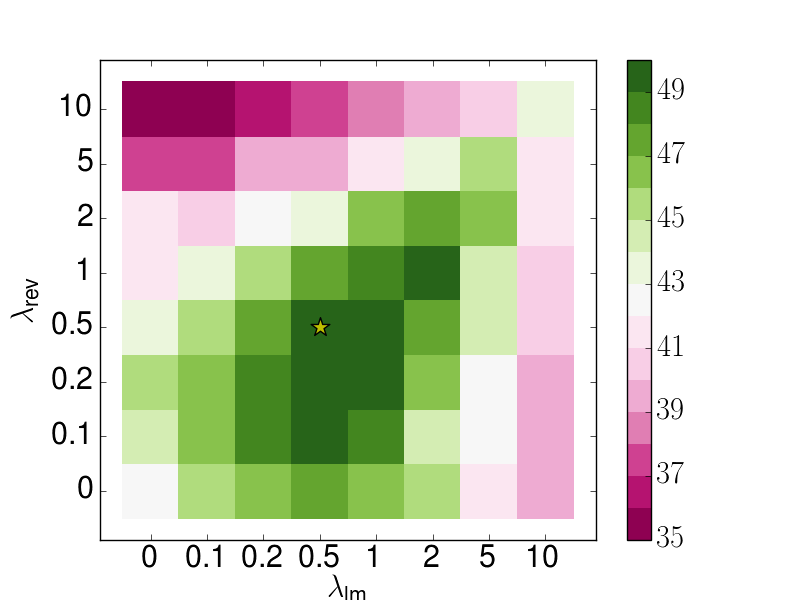
\includegraphics[scale=0.36]{0.png} & 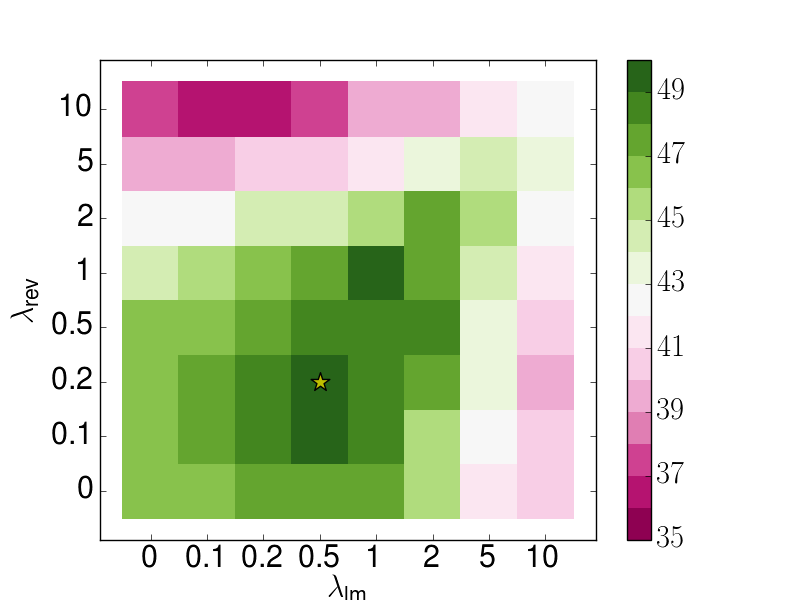
\includegraphics[scale=0.36]{1.png} \\
$\lambda_\text{fwd} = 0.1$ & $\lambda_\text{fwd} = 2$ \\
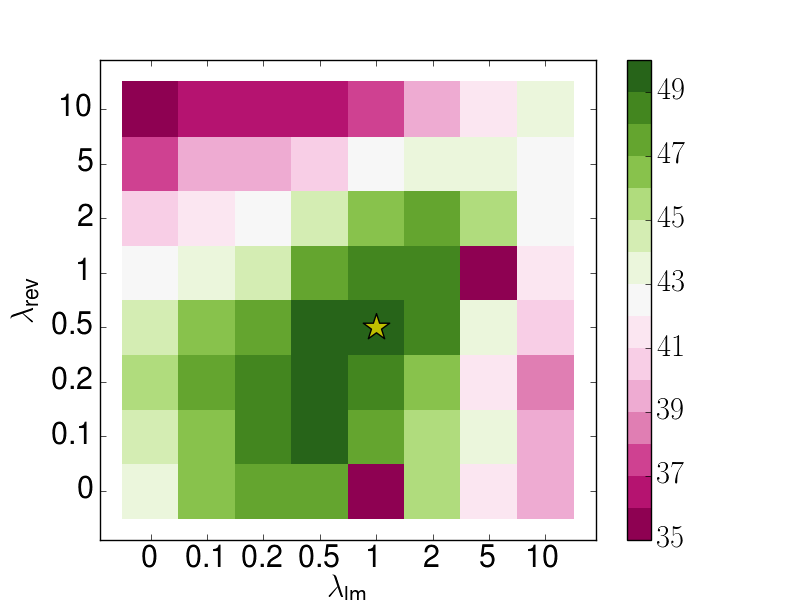
\includegraphics[scale=0.36]{0_1.png} & 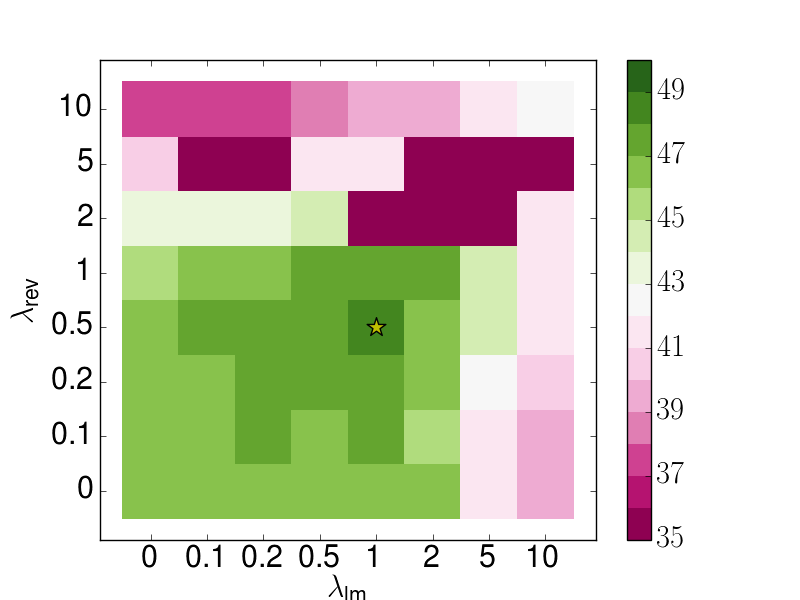
\includegraphics[scale=0.36]{2.png} \\
$\lambda_\text{fwd} = 0.2$ & $\lambda_\text{fwd} = 5$ \\
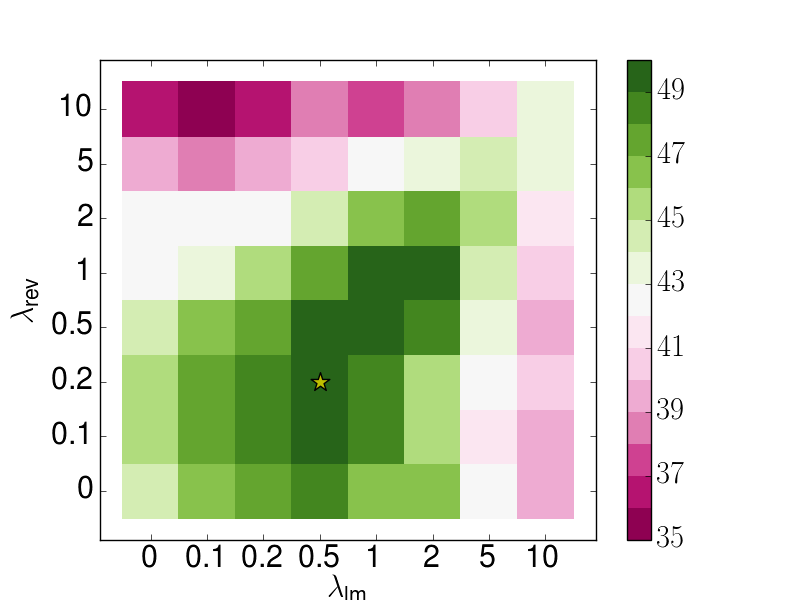
\includegraphics[scale=0.36]{0_2.png} & 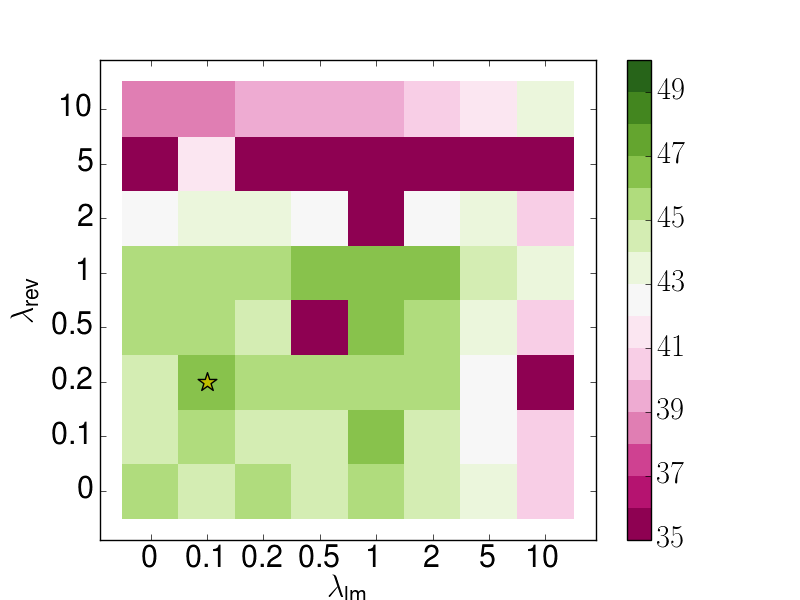
\includegraphics[scale=0.36]{5.png} \\
$\lambda_\text{fwd} = 0.5$ & $\lambda_\text{fwd} = 10$ \\
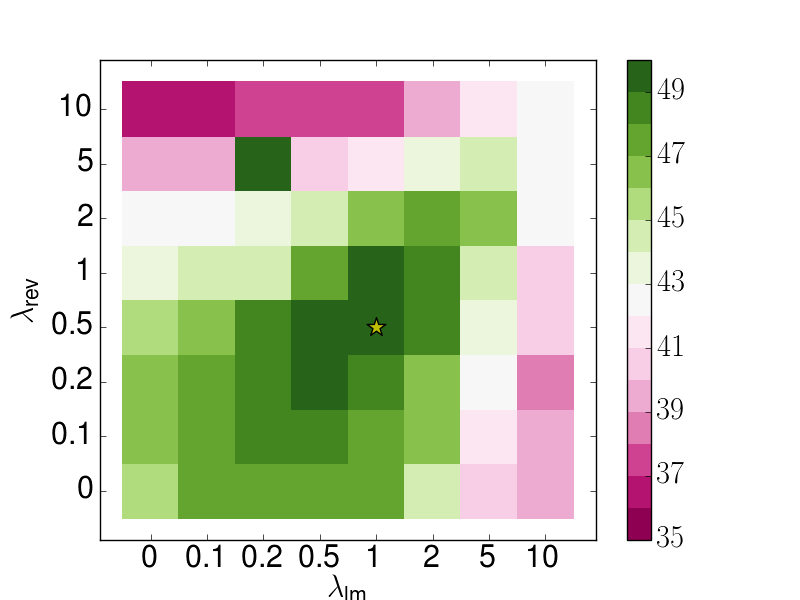
\includegraphics[scale=0.36]{0_5.png} & 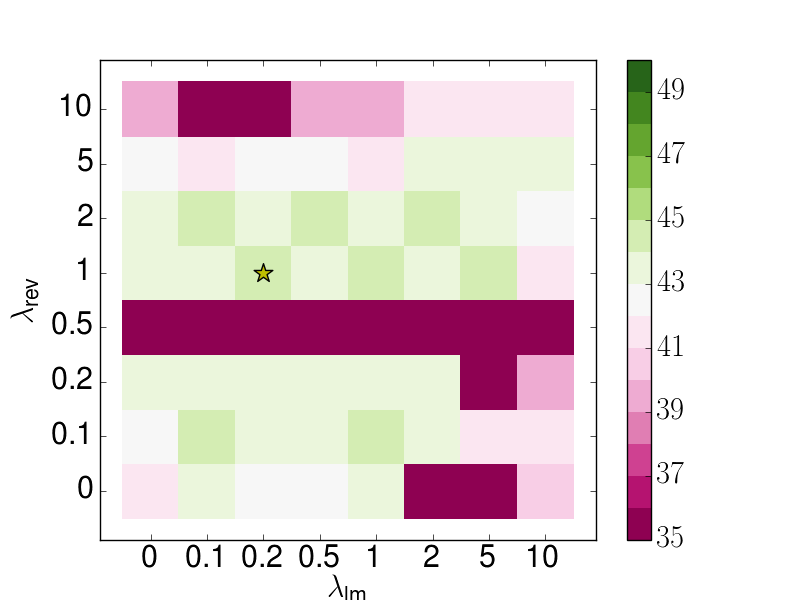
\includegraphics[scale=0.36]{10.png} \\
\end{tabular}
\caption{Plots of our grid search over $\lambda$s on BTEC. In each plot the best set of values is marked by a gold star.}
\label{fig:grid_search}
\end{figure*}

\begin{figure*}
\centering
\begin{tabular}{c c}
$\lambda_\text{fwd} = 0$ & $\lambda_\text{fwd} = 1$ \\
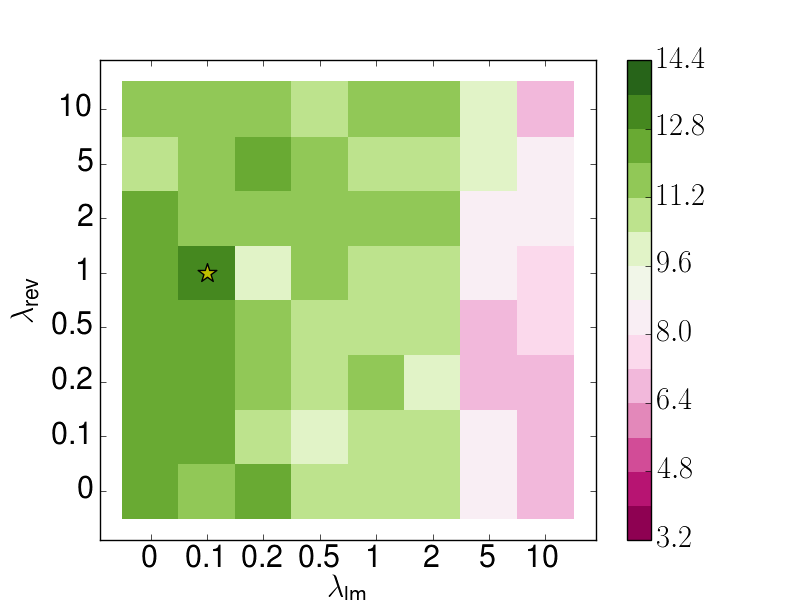
\includegraphics[scale=0.36]{wmt0.png} & 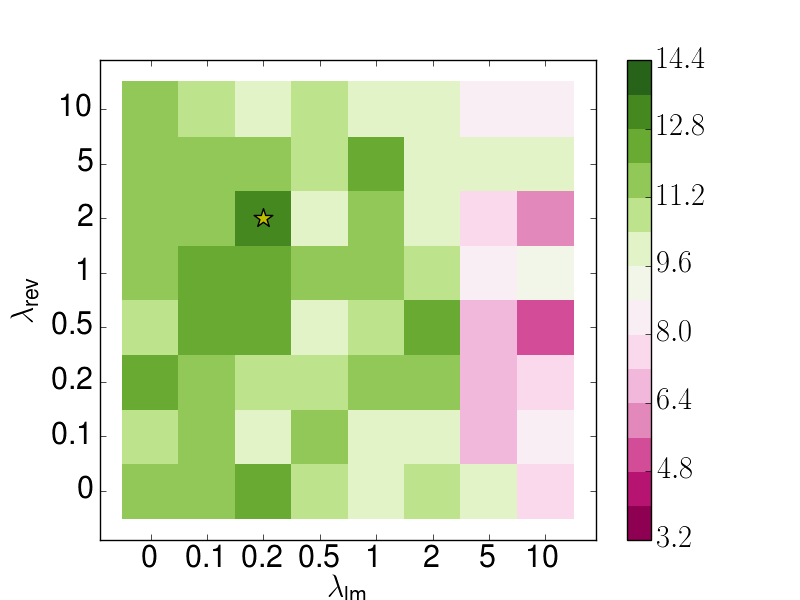
\includegraphics[scale=0.36]{wmt1.png} \\
$\lambda_\text{fwd} = 0.1$ & $\lambda_\text{fwd} = 2$ \\
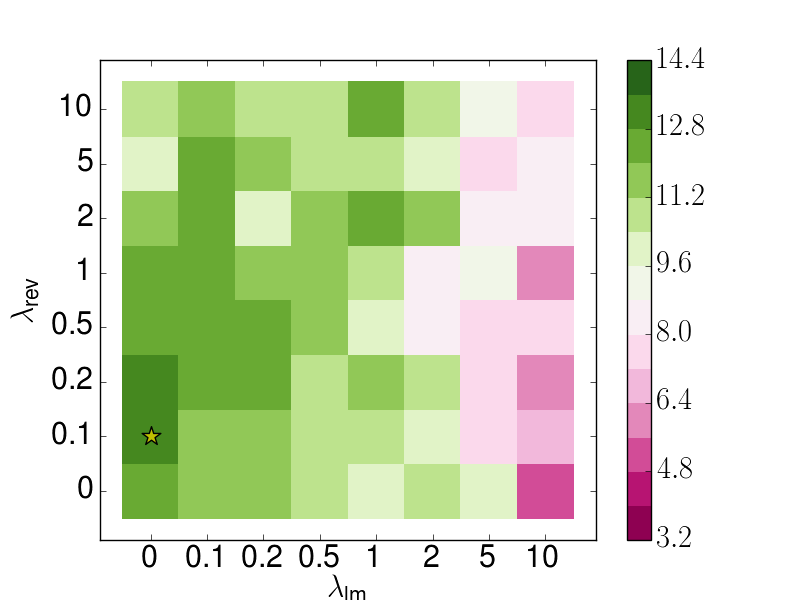
\includegraphics[scale=0.36]{wmt0_1.png} & 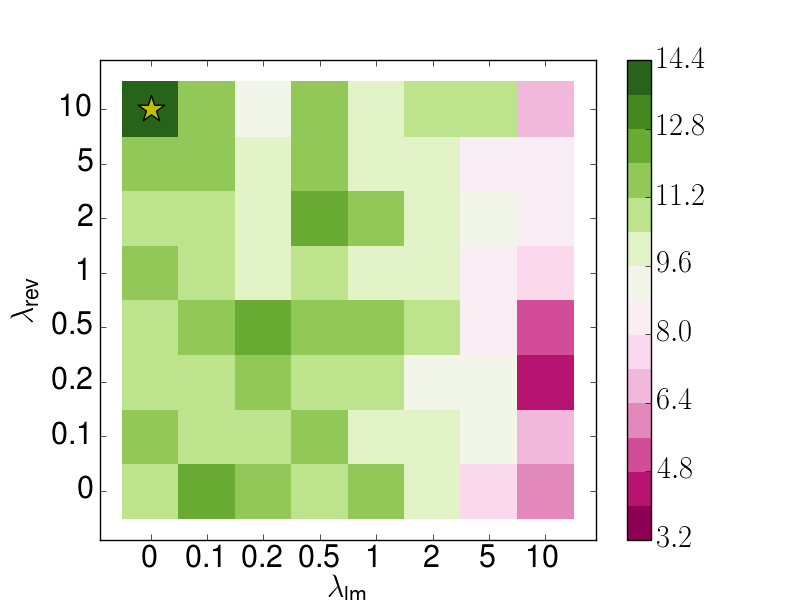
\includegraphics[scale=0.36]{wmt2.png} \\
$\lambda_\text{fwd} = 0.2$ & $\lambda_\text{fwd} = 5$ \\
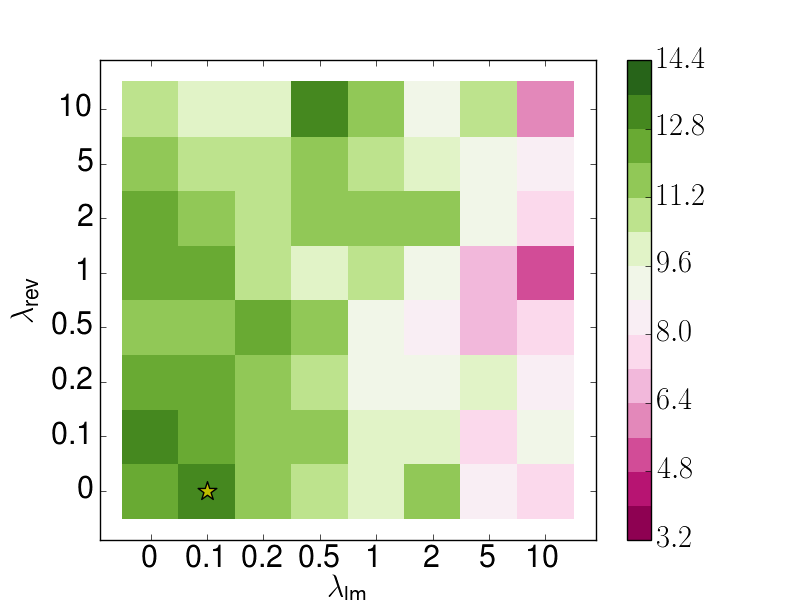
\includegraphics[scale=0.36]{wmt0_2.png} & 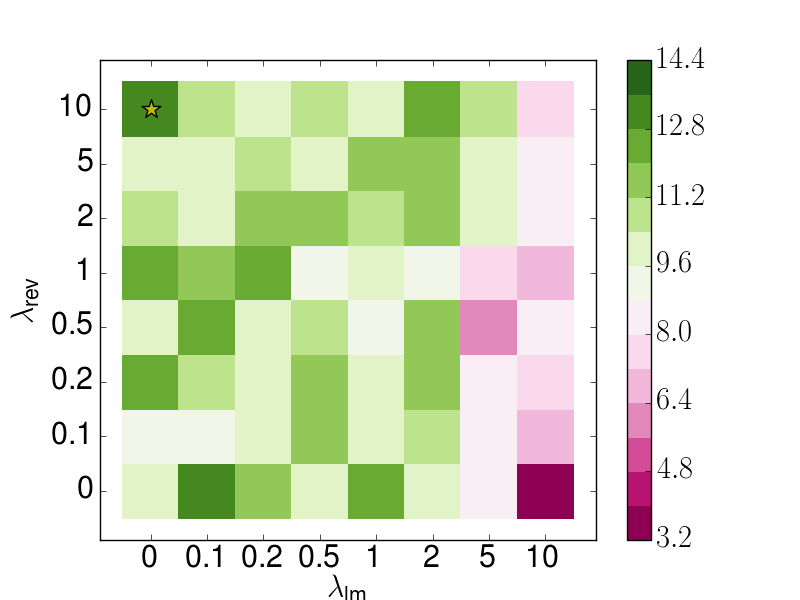
\includegraphics[scale=0.36]{wmt5.png} \\
$\lambda_\text{fwd} = 0.5$ & $\lambda_\text{fwd} = 10$ \\
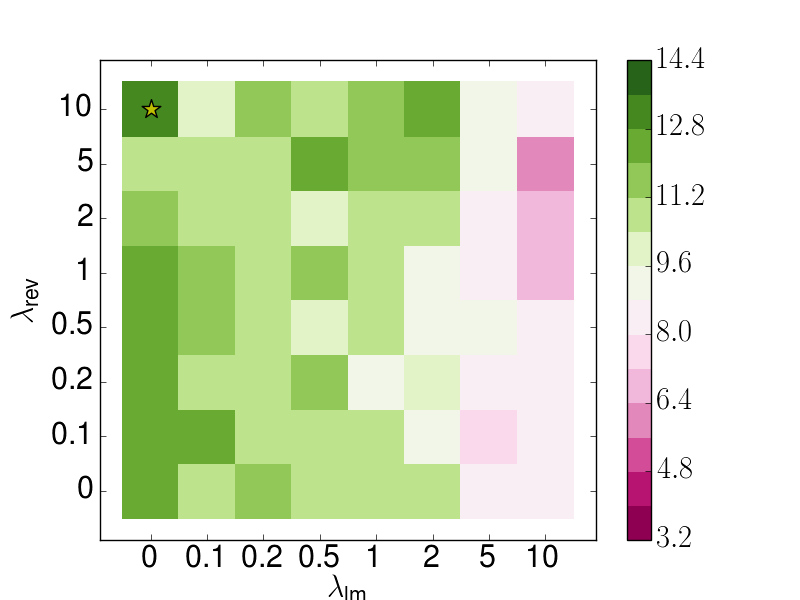
\includegraphics[scale=0.36]{wmt0_5.png} & 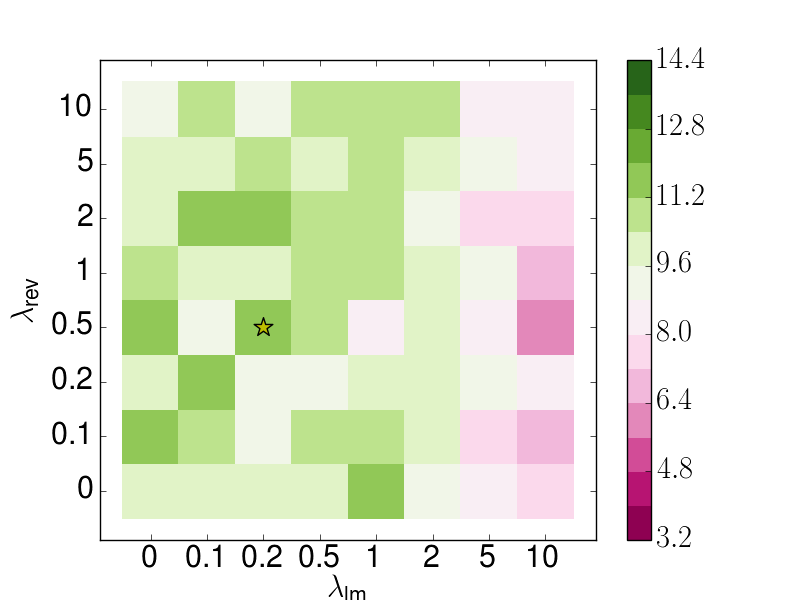
\includegraphics[scale=0.36]{wmt10.png} \\
\end{tabular}
\caption{Plots of our grid search over $\lambda$s on 30 sentences randomly sampled from the WMT dev set. In each plot the best set of values is marked by a gold star.}
\label{fig:grid_search}
\end{figure*}

The results of our grid search over $\lambda$s (using $c_\text{puct}=20$ and 200 rollouts) are visualized in Figure~\ref{fig:grid_search}.

We search over $\lambda_{\text{fwd}}$, $\lambda_{\text{rev}}$, and $\lambda_{\text{lm}} \in \{0, 0.1, 0.2, 0.5, 1, 2, 5, 10\}$
and find the optimal values to be $\lambda_\text{fwd}=0.1$, $\lambda_\text{rev}=0.5$, and $\lambda_\text{lm}=1.0$, with a BLEU score of 50.57.

%TODO: \am{Should probably also show the individual models (i.e. $p(t|s)$, $p(s|t)$, and $p(t)$)'s 1- and 16-reference BLEU scores, perplexities, etc.}

\am{WMT stuff}

\begin{table}
\centering
\begin{tabular}{r l l l l}
\toprule
& \multicolumn{2}{c}{BTEC} & \multicolumn{2}{c}{WMT} \\
\cmidrule(l{2pt}r{2pt}){2-3}\cmidrule(l{2pt}r{2pt}){4-5}
Rollouts & BLEU & Loss & BLEU & Loss \\
\midrule
1 & 32.03 & 1.17 & 6.36 & 3.21 \\
2 & 36.77 & 0.86 & 8.10 & 2.59 \\
5 & 42.32 & 0.65 & 9.06 & 2.11 \\
10 & 43.94 & 0.56 & \textbf{9.24} & 1.90 \\
20 & 44.97 & 0.50 & 9.18 & 1.74 \\
50 & 45.83 & 0.46 & 9.02 & 1.57 \\
100 & 46.06 & 0.44 & 8.76 & 1.47 \\
200 & 46.61 & 0.42 & 8.41 & 1.36 \\
500 & 46.68 & 0.41 & 7.39 & 1.29 \\
1000 & \textbf{46.75} & \textbf{0.40} & 6.58 & \textbf{1.23} \\
\bottomrule
\end{tabular}
\caption{Results with full Monte Carlo sampling on our dev sets.}
\label{tab:monte_carlo}
\end{table}

\begin{figure*}
\centering
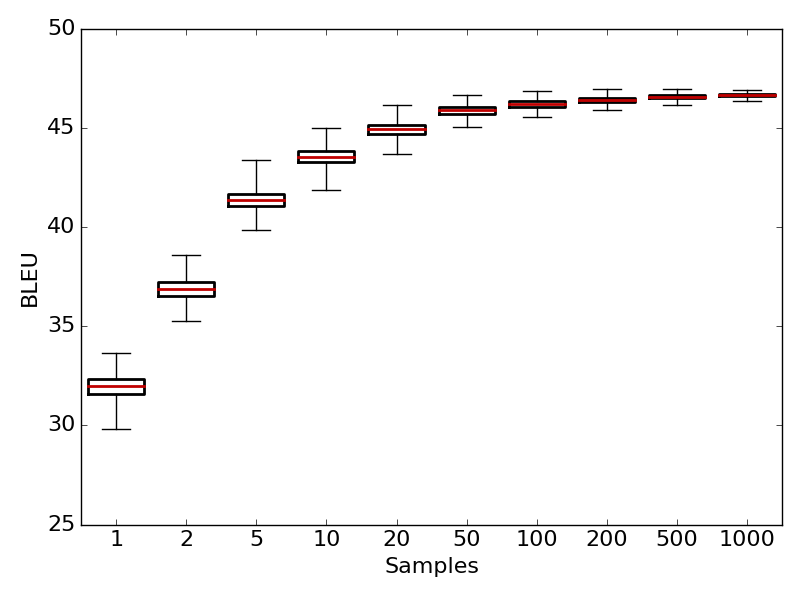
\includegraphics[scale=0.8]{mc_btec.png}
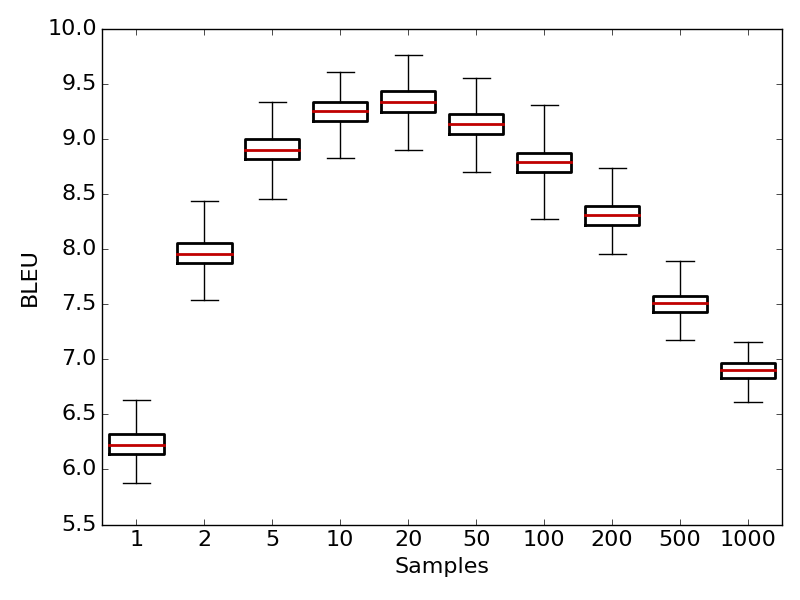
\includegraphics[scale=0.8]{mc_wmt.png}
\caption{BLEU scores with full Monte Carlo sampling on the BTEC (top) and WMT (bottom) data.}
\label{fig:monte_carlo}
\end{figure*}

\begin{figure*}
\centering
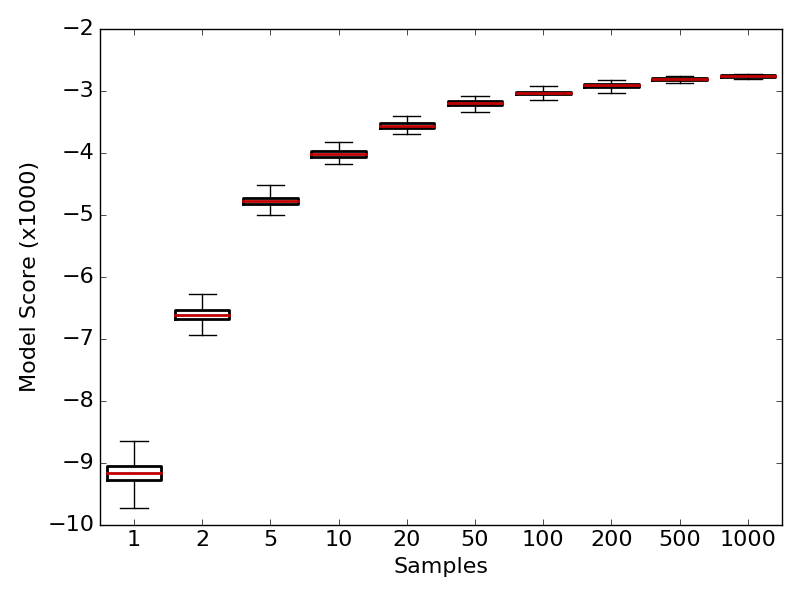
\includegraphics[scale=0.8]{ms_btec.png}
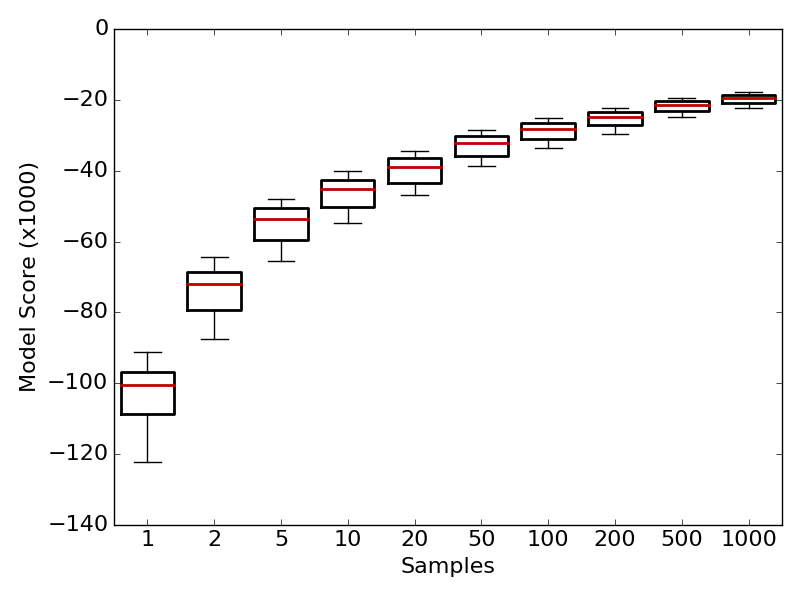
\includegraphics[scale=0.8]{ms_wmt.png}
\caption{Per sentence model scores with full Monte Carlo sampling on the BTEC (top) and WMT (bottom) data.}
\label{fig:monte_carlo}
\end{figure*}

\section{Analysis}
\label{sec:analysis}

\begin{figure*}
\centering
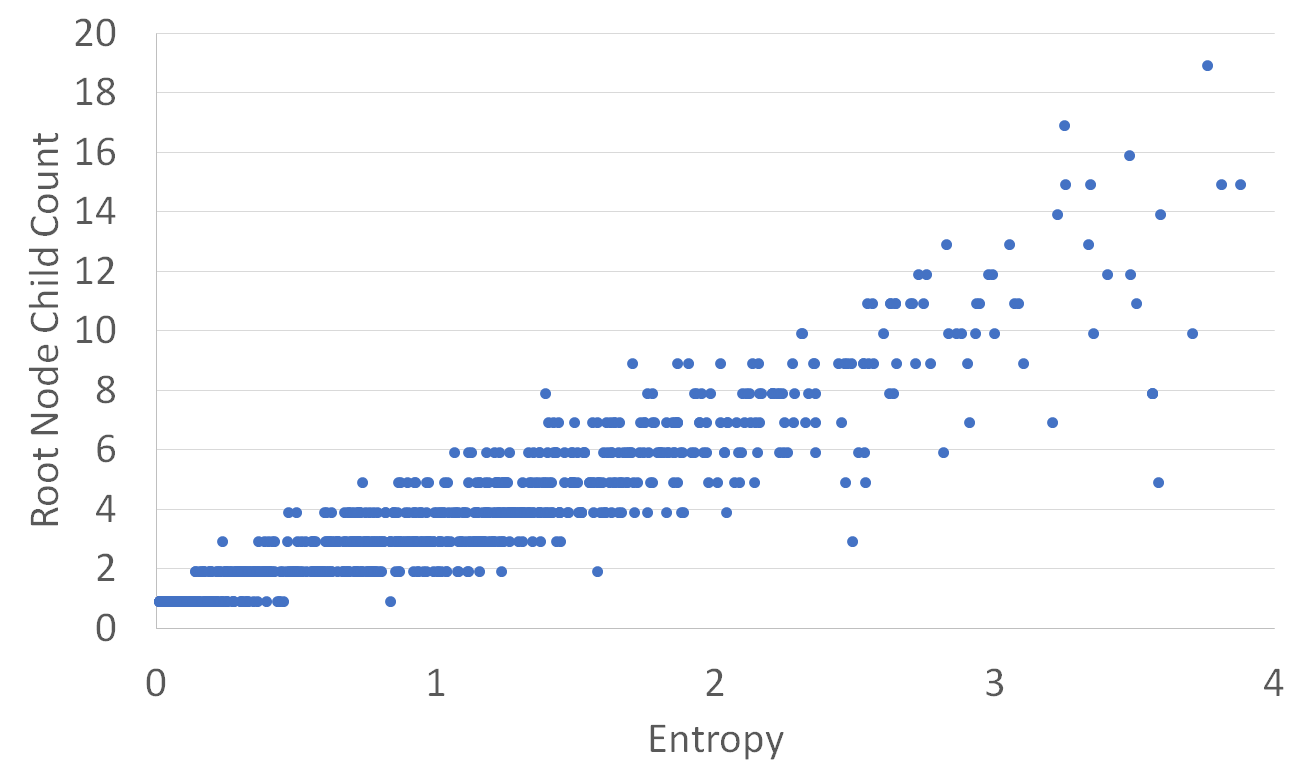
\includegraphics[scale=0.4]{branch_entropy.png}
\caption{Plot of the entropy versus the number of children (fan out) of root
nodes when decoding the BTEC ZH-EN dev set. Forward model only
($\lambda_\text{fwd}=1$, $\lambda_\text{rev}=\lambda_\text{lm}=0$), with
$c_{\text{puct}}=20$ and 200 rollouts.}

\label{fig:entropy}
\end{figure*}

We posit that the improvements from MCTS come from its ability to more
thoroughly explore interesting parts of the search space while ignoring the
less promising parts. To explore this hypothesis we examine how the branching
factor of the MCTS search changes as a function of the entropy of the
distribution output by the neural network. To avoid the effects of varying
number of visits, we limit our analysis to the root nodes of each of the 1006
sentences in our development set. The results are shown in \ref{fig:entropy}.
We can see that our algorithm explores many possible children when a node's
entropy is high and few nodes when the entropy is low. The average number of
children is 3.55 with a standard deviation of 2.78.

Since a large part of our gains comes from adding scores from additional models into our search algorithm,
it seems fair to afford beam search its closest possible approximation of that ability. Since beam search
must score partial hypotheses (and have a strictly decomposable loss), we cannot directly incorporate more than
one model into the search procedure as we can with MCTS.

\begin{table}
\centering
\begin{tabular}{r l l}
\toprule
& \multicolumn{1}{c}{BTEC} & \multicolumn{1}{c}{WMT} \\
\cmidrule(l{2pt}r{2pt}){2-2}\cmidrule(l{2pt}r{2pt}){3-3}
$k$ & BLEU & BLEU \\
\midrule
5 & - & 17.72 \\
10 & - & 17.98 \\
20 & - & TBD \\
50 & 50.52 & 17.94 \\
\bottomrule
\end{tabular}
\caption{Results of rescoring $k$ best lists using our reverse and language models}
\label{tab:rescoring}
\end{table}

Instead we produce a $k$ best list using beam search (with beam size also set
to $k$). We then compute the score of each resulting hypothesis under each of
the three models and use MERT \cite{och2003minimum} to compute optimal weights
for each on the development set. We then re-score the $k$ best lists using
these new weights and output the hypothesis that scores best under this new
weighting scheme for each sentence. The results, shown in
Table~\ref{tab:rescoring} show that this post-processing technique is able to
achieve similar gains to our MCTS ensemble. Nevertheless, we believe MCTS is
simpler, achieving these large gains in just one step as part of decoding. MCTS
also represents an exciting new approach with much more flexibility upon which
to base future research.

\section{Related Work}
\label{sec:related_work}
Other work has addressed the problem of beam search's fixed fan out without
abandoning the beam search paradigm as dramatically as we have.
\newcite{freitag2017beam} examine pruning strategies other than simply keeping
the top $k$ words at each timestep, including keeping everything within a
constant amount (either additively or multiplicatively) from the best
hypothesis.

\newcite{vijayakumar2016diverse} address the limited diversity of beam search's
outputs, a symptom of its inability to capture long-distance interactions
within hypotheses. \newcite{sun2017bidirectional} also address this
insufficiency in beam search, using a bi-directional search model. While their
bidirectional model allows for some propogation of information, but is limited
by their first-order Markov assumption.

The MCTS algorithm was originally developed for playing the game of Go
\cite{coulom2006efficient}, for which there is no known evaluation function,
and which has extremely complex long-distance interactions between moves. It
was quickly extended to simple single player games \cite{schadd2008single},
where it also showed good performance. A few years later
\newcite{maes2012monte} characterized a whole family of MCTS-based methods and
searches for the best variants on a suite of single-player games. Separately
\newcite{baier2012beam} proposed an intriguing hybrid of MCTS and Beam Search
and use it to play one-player games.

More recently \newcite{silver2016mastering} introduced neural priors into MCTS,
bringing Go AI to super-human levels for the first time. Their technique has
since been expanded to many other domains with great success \cite[inter
alia]{silver2017mastering,pinheiro2017geometric,lee2018deep,luckow2018monte}.

\section{Conclusion}
In this work we have applied Monte-Carlo Tree Search to the domain of neural
machine translation.
We have shown that MCTS can compete with beam search and admits exciting new
possibilities for searching with a diverse set of models.
We have demonstrated gains on two language pairs, with small gains just from
changing the search algorithm and large gains from using an ensemble of a
forward translation model, a reverse translation model, and a language model.

\section*{Acknowledgements}
\label{sec:acknowledgements}
Google for letting us use Borg.
Matthias for help with LMs in xnmt.

\bibliography{biblio}
\bibliographystyle{acl_natbib_nourl}

\appendix

\end{document}
